
\documentclass{llncs}

\usepackage{url}
\usepackage{graphics}

\newcommand{\workingnote}[1]{}        % The version that hides the note.
%\newcommand{\workingnote}[1]{(**#1)}   % The version that makes the note visible.

%\newif\ifpdf
%\ifx\pdfoutput\undefined
%   \pdffalse
%\else
%   \pdfoutput=1
%   \pdftrue
%\fi

\begin{document}
%\setstretch{2.0}

%% Use dvipdfm instead. --DH
%\ifpdf
%  \pdfcompresslevel=9
%  \pdfpagewidth=\the\paperwidth
%  \pdfpageheight=\the\paperheight
%\fi

\title{The Mixminion Anonymous Remailer}
\author{George Danezis\inst{1} \and Roger Dingledine\inst{2} \and Nick Mathewson\inst{2}}
\institute{Cambridge
\email{(george.danezis@cambridge)}
\and
The Free Haven Project
\email{(arma@mit.edu)}
% add some more people here
}
\maketitle
\pagestyle{empty} 
  
\begin{abstract}

We describe a packet-based anonymous remailer protocol which supports
secure single-use reply blocks and includes link-level encryption to provide
forward anonymity. We describe designs for directory servers and nymservers,
and discuss their anonymity implications. We include justification
for various design decisions and a detailed description of attacks and
defenses. And some other stuff.

\end{abstract}

Keywords: anonymity, peer-to-peer, remailer, store-and-forward, reply block %, ...

%%%%%%%%%%%%%%%%%%%%%%%%%%%%%%%%%%%%%%%%%%%%%%%%%%%%%%%%%%%%%%%%%%%%%%%

\section{Introduction}
\label{sec:intro}

Chaum first introduced anonymous remailer designs over 20 years ago
\cite{chaum-mix}. The research community has since introduced many new
designs and proofs \cite{big chain of cites?}, and discovered a variety
of new attacks \cite{more cites?}, but the
state of deployed remailers has changed remarkably little since Cottrell
published his Mixmaster software \cite{mixmaster-attacks} eight years
ago. Part of the difficulty in expanding the deployed remailer base is
due to the liability involved in running a remailer node on the Internet,
and part is due to the complexity of the current infrastructure ---
it is very hard to add new experimental features to the current software.

The Mixminion project aims to deploy a cleaner updated remailer design
in the same spirit as Mixmaster, with the goals of expanding deployment,
documenting our design decisions and how well they stand up to all known
attacks, and providing a research base for experimental features. We
describe our overall design in Section \ref{sec:design}, including two
designs for a new primitive called a \emph{single-use reply block}
(SURB).  Mixmaster provides no support for replies, instead relying
on the older and less secure cypherpunk type I remailer design
\cite{cypherpunk-remailer}. By integrating reply capabilities into
Mixminion, we can finally retire the type I remailer network.

We go on in Section \ref{sec:dir-servers} to describe a design for
Directory Servers to track and distribute remailer availability,
performance, and key information, and then describe in Section
\ref{sec:nymservers} how to build higher-level systems such as nymservers
using SURBs. We introduce link-level encryption with ephemeral keys to
ensure forward anonymity for each message. We also provide flexible
delivery schemes --- rather than just allowing delivery to mail or
usenet, we allow designers to add arbitrary modules to handle incoming
messages. By separating the core mixing architecture from these
higher-level modules, we can limit their influence on the anonymity
properties of the system.

Mixminion aims to be a best-of-breed remailer which uses conversative
design approaches to provide security against most known attacks.
Many of our design decisions impacted anonymity in surprising ways. Herein
we document and analyze some of these influences to provide more intuition
to developers and users.

%%%%%%%%%%%%%%%%%%%%%%%%%%%%%%%%%%%%%%%%%%%%%%%%%%%%%%%%%%%%%%%%%%%%%%%

\section{Related Work}

\subsection{MIX-nets}

Chaum introduced the concept of a MIX-net for anonymous communications
\cite{chaum-mix}. A MIX-net consists of a group of servers, called MIXes
(or MIX nodes), each of which is associated with a public key. Each
MIX receives encrypted messages, which are then decrypted, batched,
reordered, stripped of the sender's name and identifying information, and
forwarded on. Chaum also proved security of MIXes against a \emph{passive
adversary} who can eavesdrop on all communications between MIXes but is
unable to observe the reordering inside each MIX.

Current research directions on MIX-nets include ``stop-and-go'' MIX-nets
\cite{kesdogan}, distributed ``flash MIXes'' \cite{flash-mix} and their
weaknesses \cite{desmedt,mitkuro}, and hybrid MIXes \cite{hybrid-mix}.

\subsection{Deployed Remailer Systems}

The first widespread public implementations of MIXes were produced by the
cypherpunks mailing list. These ``Type I'' \emph{anonymous remailers}
were inspired both by the problems surrounding the {\tt anon.penet.fi}
service \cite{helsingius}, and by theoretical work on MIXes. Hughes wrote
the first cypherpunks anonymous remailer \cite{remailer-history}; Finney
followed closely with a collection of scripts which used Phil Zimmermann's
PGP to encrypt and decrypt remailed messages. Later, Cottrell implemented
the Mixmaster system \cite{mixmaster}, or ``Type II'' remailers, which
added message padding, message pools, and other MIX features lacking
in the cypherpunk remailers. At about the same time, Gulcu and Tsudik
introduced the Babel system \cite{babel}, which also created a practical
remailer design (although one that never saw widespread use).

\subsection{Remailer Statistics}

Levien's \emph{statistics pages} \cite{levien} track both remailer
capabilities (such as what kinds of encryption the remailer supports)
and remailer up-times, observed by pinging the machines in question
and by sending test messages through each machine or group of machines.
Such \emph{reputation systems} improve the reliability of MIX-nets by
allowing users to avoid choosing unreliable MIXes. The Jack B Nymble 2
remailer client \cite{potato} allows users to import statistics files
and can then pick remailers according to that data. Users can specify
minimum reliability scores, decide that a remailer should always or never
be used, and specify maximum latency. Ongoing research on more powerful
reputation systems includes a reputation system for free-route networks
\cite{mix-acc} and a more secure one for MIX cascades \cite{casc-rep}.

% maybe add a subsection on nymservers too?

%%%%%%%%%%%%%%%%%%%%%%%%%%%%%%%%%%%%%%%%%%%%%%%%%%%%%%%%%%%%%%%%%%%%%%%

%\section{Goals and Assumptions}
% covered below, at least in part.

% and non-goals
% threat models, etc

%http://archives.seul.org//mixminion/dev/Mar-2002/msg00004.html
%http://archives.seul.org//mixminion/dev/Mar-2002/msg00014.html

%%%%%%%%%%%%%%%%%%%%%%%%%%%%%%%%%%%%%%%%%%%%%%%%%%%%%%%%%%%%%%%%%%%%%%%

\section{Design Overview}
\label{sec:design}

Mixminion aims to bring together the current best approaches for providing
anonymity in a batching message-based MIX environment. We don't aim
to provide low-latency connection-oriented services like Freedom
\cite{freedom} or Onion Routing \cite{onion-routing} --- while those
designs are more effective for common activities like anonymous web
browsing, it seems they cannot provide the level of strong anonymity of
slower message-based services [Do we, uh, want to cite that?]. Indeed, we
further intentionally restrict the set of options for users: we provide
only one cipher, and we avoid extensions that would help an adversary
divide the anonymity set.

We chose to drop backward-compatibility with Mixmaster and the cypherpunk
remailer systems, in order to provide a simple extensible design. At
the same time, we provide a new feature: a reply block mechanism which
is as secure as forward messages.

Reusable reply blocks are security risks --- by their very nature they
let people send multiple messages to them. These multiple messages can be
used to very quickly trace the recipient's path: if two incoming batches
both include a message to the same reply block, then the next hop must
be in the intersection of both outgoing batches.

%Mixmaster solves the problem by not providing reply functionality,
%and instead falling back on the less secure multiple-use reply blocks
%provided by the type I remailer network.

The rest of this section describes the header structure and the
protocol for building and processing messages. In particular, we
focus on two competing ways of providing secure reply functionality,
and the tradeoffs and design decisions surrounding each approach. In
the first approach, we provide a mechanism for doing replies where a
reply message is indistinguishable from a forward message. Because this
approach introduces some attacks which we cannot adequately address, we
then propose a second approach which allows forward and reply messages
to be distinguished but provides better overall security.


\subsection{Approach one: the `header swap' method}
\label{subsec:header-swap}

Making forwards and replies indistinguishable prevents an adversary from
dividing the message anonymity sets into two classes. In particular, if
there are very few replies during a given period relative to the total
number of messages, an adversary controlling some of the MIXes in the
network can more easily trace the path of each reply --- even though
the batches may be large, the number of replies in each batch will be
quite small.

At the same time, protocols like Mixmaster include hashes of the entire
message in each header. Each hop in the path checks the integrity of
the header and payload, and drops the message immediately if it's been
altered. But since the author of the reply block is not the one writing
the payload, these hashes can no longer be used. Indeed, since we choose
to make forward message and replies indistinguishable, we cannot provide
hashes for forward messages either. This choice introduces a new class
of attacks known as \emph{tagging attacks}.

\begin{figure}
\begin{center}
\resizebox{10cm}{!}{\includegraphics{SWAP.eps}}
\caption{The operations requered by the ``swap'' method} 
\end{center}
\end{figure}

The ``header swap'' mechanism could be used in order to minimize the
information leaked by \emph{tagging attacks}. Each mixminion packet,
when created, has two headers: the first one contains a series of sub
headers encrypted as an onion under the public keys of a sequence of
nodes. Each of these sub headers contain some symmetric key and a hash
to check the integrity of the header. The second header contains sub
headers in the form of an onion as well but is also encrypted under
the keys contained in the first header, as well as the hash of the
payload. The second header could also be a single use reply block (SURB)
provided by another party. The payload is finally encrypted using all
the keys contained in the first header and the second if it is not a SURB.

The packet travels through nodes that perform the operations illustrated
on \emph{figure 1}. Each node decrypts the RSA sub header, retrieves
the key and checks the integrity of the first header. If someone has
tampered with it, the packet is discarded. If the header is correct,
the secret is used to decrypt the second header and the payload. The
is one special node, at the ``crossover point'', in the path that in
addition to the standard operation, decrypts the second header using
the hash of the payload and swaps the two headers.

The primitive used for encryption and decryption is BEAR \cite{BEAR},
a variable block size block cipher. It offers the property that if any
bit of the encrypted material is changed the decryption will look like
random bits for anyone that does not know the key. Therefore we minimize
an attackers benefit for tagging the message. It is impossible to tag the
headers because any modification is detectable. It is also fruitless to
modify the payload of the message: if it is modified before the crossover
point, the second header will not be decryptable, and if it is modified
afterward the first part of the path should offer enough anonymity. Of
course in order to make this scheme as secure as if tagging attacks did
not exist we should require users to choose the double path length for
each message. In practice users might choose to select shorter paths,
given that the tagging attack provides very little information and is
very difficult to mount.

\subsection{Approach two: the `distinguish replies' method}
\label{subsec:distinguish-replies}

%David? :)

\subsection{Link-level encryption and what it gets us}

Unlike remailer types I and II that used SMTP as their underlying
transport mechanism, Mixminion clients and nodes communicate using a
forward secure encrypted channel based on TLS \cite{TLS}.  TLS allows
the establishment of an encrypted tunnel using ephemeral
Diffie-Hellman keys. In order to make sure that the receiving end is
the one intended by the creator of the anonymous message, the
ephemeral key could be signed by the receiving node. As soon as a
session key has been established the Diffie-Hellman keys are destroyed
and messages start being sent through the tunnel. After each message a
standard key update operation is performed to generate a new key and
the old key material is deleted. Key updates don't use any asymmetric
encryption techniques, so they are quite fast.

The above scheme offers forward secrecy in the sense that even the
nodes that exchange messages are not able to decrypt or even recognize
messages that might have been intercepted on the links. This makes it
impossible to comply with decryption notices that might be served in
some jurisdiction.  It also makes it necessary for an adversary to
corrupt and control nodes in order to have enough information to trace
back a forward anonymous communication by requesting nodes to decrypt
it. (Reply blocks can still be used for this purpose.)  Even if an
attacker manages to get hold of the session key at a particular point
they would have to observe all subsequent traffic to be able to update
their key appropriately.

The forward secure encrypted channel offers only limited protection
against traffic analysis. Encrypted links between honest nodes prevent
an adversary from recognizing even his own messages; but without
link padding, he is still able to measure how much traffic is being
transmitted.
%and its recipient.

\subsection{Message types and delivery modules}

Once a Mixminion packet reaches the final MIX in its path, it must be
dropped (if it is a dummy message), or delivered to its intended
recipient (if it is not).  In order to support different kinds of
delivery, each header contains a type code for the action to be taken
to deliver the message.  A few types--such as DUMMY, SMTP, and LOCAL
DELIVERY--are specified as a part of the Mixminion standard.  Others
may be added by future extensions, in order to implement
abuse-resistant exit policies (see \ref{subsec:exitpolicies}), to
administer nymservers (see \ref{subsec:nymservers}), to publish
anonymously to USENET, or to support other protocols.

% We never reached a consensus (afaik) on whether 'FORWARD' and 'DROP'
% were types or not.  Are they? -Nick

Nearly all delivery methods require additional information beyond the
message type and its payload.  The SMTP module, for example, requires
an email address.  In our current design, this information is placed
in a variable-length annex to the final header.  \footnote{It must be
in the header, since putting delivery information in the payload would
prevent people from creating SURBs that delivered by SMTP.  On the one
hand, under the ``header swap'' method described in
\ref{subsec:header-swap), the all-or-nothing property of BEAR prevents
generator of a reply block from putting any information in the
payload.  On the other hand, under the ``distinguish replies'' method
in \ref{subsec:distinguish-replies}, the delivery information would
create a portion of the payload that the final node {\it could}
distinguish from random garbage, thus allowing a tagging attack
against the reply block.}
% See my messages of April 9 and 10 titled ``SMTP service'' for a more
% detailed version of the above argument. -Nick
%
% Should we say _why_ it's undesirable to force reply recipients to
% run local nodes?  [My answer is (A) that some people (such as human
% rights activists using internet cafes) want to get replies, but
% don't have persistant net connections, (B) that Mixmaster
% supports it, and not doing so would be a step backwards, and (C)    
% that there's not much reason not to.]    -Nick

The types each MIX supports are described in a \emph{capability
block}, which also includes the MIX's address, long-term (signing)
public key, short-term key (for use in header encryption), and
forwarding strategy (if any).  MIXes sign these capability blocks, and
publish them on directory servers (see \ref{sec:dir-servers}).
Clients download this information from the directory servers.

% Is all of the stuff above really in the caps block?  Or do we break
% the volatile part (short-term key) from the nonvolatile part? -Nick

The possibility of multiple delivery methods doesn't come free: their
presence may fragment the anonymity set.  For example, if there were 5
ways to send a SMTP message to Bob, an attacker could partition Bob's
incoming mail by assuming that one of those ways was Alice's favorite.
Furthermore, an active attacker Mallory could lure users into using an
exit node he had compromised by advertising that node as supporting a
rare but desirable delivery method.

We claim that these attacks do not provide an argument against
extensibility _per se_, but rather argue against the proliferation
of redundant extensions, and against the use of rare extensions.  

\subsection{Exit policies and abuse}
\label{subsec:exitpolicies}

One important entry in a node's capability block is its \emph{exit
policy}. Exit abuse is a serious barrier to wide-scale remailer deployment
--- rare indeed is the network administrator tolerant of machines that
potentially deliver hate mail to the President.

On one end of the spectrum are \emph{open exit} nodes which will
deliver anywhere; on the other end are \emph{middle-man} nodes which
only relay traffic to other remailer nodes. More generally, nodes can
set individual exit policies to declare which traffic they will let
exit from them, such as traffic for local users or other authenticated
traffic \cite{onion-discex00}.

Preventing abuse of open exit nodes is an unsolved problem. If
receiving mail is opt-in, an abuser can forge an opt-in request from
his victim. Indeed, requiring recipients to declare their interest
in receiving anonymous mail is risky --- human rights activists in
Guatemala cannot both sign up to receive anonymous mail and also retain
plausible deniability.\footnote{
  Compare with the 1965 U.S. Supreme Court case Lamont v. Postmaster
  General (381 U.S. 301), where the Post Office would detain mail it
  deemed to be `communist political propaganda' and instead send a form
  to the addressee telling him to send back the signed form if he wanted
  to receive such mail. The government maintained a list of citizens
  who had filled out these forms.
} Similarly, if receiving mail is opt-out, an abuser can deny service
by forging an opt-out request from a legitimate user. We might instead
keep the mail at the exit node and send a note to the recipient
informing telling them how to collect their mail; but this increases
server liability by storing messages (see \ref{sec:nymservers} below),
and also doesn't really solve the problem.

Of course, a mixture of open and restricted exit nodes will allow the
most flexibility for volunteers running servers. But while a large number
of middle-man nodes is useful to provide a large and robust network, the
small number of exit nodes still simplifies \emph{traffic confirmation}
(attacks where the adversary observes both a suspected user and the
network's exit nodes and looks for timing or packet correlations). The
number of available open exit nodes remains a limiting security parameter
for the remailer network.

%%%%%%%%%%%%%%%%%%%%%%%%%%%%%%%%%%%%%%%%%%%%%%%%%%%%%%%%%%%%%%%%%%%%%%%

\section{Directory Servers}
\label{sec:dir-servers}

Although the current Mixmaster protocol does not specify a means for
clients to learn the locations, keys, capabilities, or performance
records of participating mixes, several schemes have been implemented
\cite{mix-stats} and adopted by some clients.  As an adjunct the
Mixminion protocol, we specify such a system.

We begin by discussing some attacks that system of directory servers
must address, and then propose a secure but inefficient design.

\subsection{Directory-related attacks}
\label{subsec:dir-server-attacks}

A fairly broad category of vulnerabilities stems from the fact that
knowledge among clients changes over time, and an adversary's ability
to create or exploit such changes.

In the most simple attack, an adversary who controls a directory
server can provide a different information to clients it wishes to
track.  For example, the compromised server might only list MIXes
controlled by the adversary; or only inform certain clients about a
given MIX. 

Even without control of the a directory server, an adversary can still
exploit differences among client knowledge.  If Eve knows that MIX M
is listed on server D1 but not on D2, she can use this knowledge to
link traffic through M to clients who have queried D2.  Eve can also
distinguish traffic based on any differences between clients who use
directory servers and those who don't; between clients who have
up-to-date listings and those who have old listings; and (if the
directory is partitioned) between clients who have different subsets
of a complete directory.  In fact, even if Eve does not know the exact
difference between Alice's knowledge and Bob's, the presence of such a
difference can aid her traffic analysis. [[CAN WE HAVE A CITE HERE?]]

Even with no differences in client knowledge, an attacker can mount a
more subtle attack by delaying messages in a comprimised MIX.  If
Alice sends a message at noon to a MIX controlled by Mallory, and he
delays the message until directory servers remove some MIX M from
their listings, he can conclude that any messages that are still
addressed to M are likely to have originated from Alice's message.  If
Mallory controls a large set of nodes, and can arrange for a large
number of them to become unlisted, he can mount this attack with a
fair probability of success. [[CAN WE DOCUMENT THIS?]]

\subsection{A Directory Service for Mixminion}
\label{subsec:dir-server-design}

As we describe above, it is not merely a matter of convenience for
clients to retrieve up-to-date MIX information; if some client
software supports a static list of servers while other software is
dynamic, this difference can help an attacker distinguish their
traffic.  Thus, we must specify a directory service as a part of our
standard.

In the most basic design, we provide protocols for MIXes to advertise
themselves to directory servers, and for clients to download
\emph{complete} directories,
  \footnote{We have considered, and rejected for performance reasons, 
            PIR-based \cite{PIR} approaches that would allow clients
            to retrieve a subset of the directory without the
            server learning which subset.} 
either directly or anonymously.  To prevent differences in client
knowledge, servers must synchronize with one another, and must only
update their exported data nightly.

To mitigate the effects of changeover, clients should download new
information regularly, but wait for a given time threshold (say, an
hour) before using any newly-published nodes.  To address delaying
attacks, clients should continue sending dummy traffic to de-listed
nodes. [[IS THIS RIGHT?]]

Directory servers compile availability information by sending traffic
through MIXes in their directories. [[NEED TO SAY MORE.]] Future
designs may include more sophisticated measures of reliability.

We do not currently specify a means to detect and blacklist
misbehaving directory servers.  Because the set of such servers is
smaller and more static than the set of nodes, we have some hope for
out-of-band detection.  Additionally, servers can work together to
ensure correct and complete data by successively signing certificate
bundles, so users can be sure that a given mix certificate has been
seen by a threshold of directory servers.


% See http://archives.seul.org/mixminion/dev/Apr-2002/msg00002.html

%%%%%%%%%%%%%%%%%%%%%%%%%%%%%%%%%%%%%%%%%%%%%%%%%%%%%%%%%%%%%%%%%%%%%%%

\section{Nym management and single-use reply blocks}
\label{sec:nymservers}

Current nymservers, such as {\tt nym.alias.net} \cite{nym-alias-net},
maintain a set of \{email address, reply block\} pairs to allow users to
receive mail without revealing their identities. When mail arrives to {\tt
bob@nym.alias.net}, the nymserver attaches the payload to the associated
reply block and sends it off into the mix-net. Because these nymservers
use the type I remailer network, these reply blocks are \emph{persistent}
or \emph{long-lived} nyms --- the mix network does not drop replayed
messages, so the reply blocks can be used again and again. Reply block
management is much simpler in this model because users only need to
replace a reply block when one of the nodes it uses stops working.

The Mixminion design protects against replay attacks by dropping
messages with repeated headers --- so its reply blocks are necessarily
single-use. There are a number of approaches for building nymservers
when reply blocks are single-use.

The approach most similar to currently deployed nymservers involves
keeping a set of reply blocks around and using one for each incoming
message. As long as the owner of the pseudonym keeps the nymserver
well-stocked, no messages will be lost. But it's hard to know at what
rate to supply the nymserver with new nyms; indeed, this approach is
vulnerable to a DoS attack to use up all the available reply blocks and
block further messages from getting delivered.

A more robust design uses an imap-like protocol: messages arrive and queue
at the nymserver, and the user periodically checks the status of his mail
and sends a sufficient batch of reply blocks so the nymserver can deliver
that mail. The above flooding attack still works, but now it's exactly
like flooding a normal imap mailbox, and the usual techniques (e.g.,
allowing the user to delete mails at the server or specify which mails to
download and let the others expire) work fine. The user can send a set
of hashes or other indices to the server after successfully receiving
some messages, to indicate that those messages can now be deleted.

Of course, there are different legal and security implications for the two
designs. In the first case, no mail is stored on the server, but it's also
keeping valid reply blocks on hand. The second case is in some sense more
secure but also creates more liability --- the server has no valid reply
blocks on hand in general, but it has to keep mail for each recipient
until it's retrieved. The owner of the pseudonym could provide a public
key which the nymserver uses to immediately encrypt all incoming messages,
to limit the amount of time the nymserver keeps plaintext messages.

Which point on the spectrum is best depends on the situations and
preferences of the volunteers running the nymservers. Hopefully there
will be enough volunteers that users can choose the set-up that makes
them most comfortable.

%%%%%%%%%%%%%%%%%%%%%%%%%%%%%%%%%%%%%%%%%%%%%%%%%%%%%%%%%%%%%%%%%%%%%%%

\section{Maintaining anonymity sets}

\subsection{Long-term nyms: how to choose paths for reply blocks}

This question is hard. We're going to have to argue about it for a
while more, I think.

\subsection{Transmitting large files with Mixminion}

http://archives.seul.org/mixminion/dev/Apr-2002/msg00031.html

\subsection{key rotation, message expiration, and replay attacks}

Mixmaster offers rudimentary replay prevention by keeping a list of recent
message IDs. To keep the list from getting too large, it expires entries
after a user-configurable amount of time. But if an adversary records
the input and output batches of a mix and then replays a message after
the mix has forgotten about it, the message's decryption will be exactly
the same. Mixmaster does not provide the forward anonymity that we want.

Chaum first observed this attack in \cite{chaum-mix}, but his solution
--- include in each message a timestamp that describes when that message
is valid --- also has problems. Specifically, it introduces a new class
of \emph{partitioning} attacks, where the adversary can distinguish and
track messages based on timestamps. If messages have short lifetimes,
legitimate messages may arrive after their expiration date and be
dropped. But if we specify expiration dates well after when we expect the
message to arrive, messages arriving near their expiration date will be
rare: an adversary can delay a message until near its expiration date,
then release it and trace it through the network.

%More generally, these partitioning attacks arise whenever a message can be
%`very rare' and `valid' at the same time.

One way of addressing this partitioning attack is to add dummy traffic
so it's less rare for messages to arrive near their expiration date;
but dummy traffic is still not well-understood. Another approach would
be to add random values to the expiration time of each mix in the path,
so an adversary delaying a message at one mix could not expect that it
is now near to expiring elsewhere in the path; but this seems open to
statistical attacks.

Mixminion provides a compromise solution that hopefully avoids many of
these problems while still providing forward anonymity. Messages don't
contain any timestamp or expiration information. Each mix must keep
hashes of the headers of all messages it's processed since the last time
it rotated its key. Mixes should choose key rotation frequency based on
security goals and on how many hashes they want to be remembering.

Note that this solution doesn't entirely solve the partitioning problem
--- near the time of a key rotation, the anonymity set of messages will
be divided into those senders who knew about the key rotation and used
the new key, and those who didn't.

%%%%%%%%%%%%%%%%%%%%%%%%%%%%%%%%%%%%%%%%%%%%%%%%%%%%%%%%%%%%%%%%%%%%%%%

\section{Implementation choices}
\label{sec:implementation}

some details about how to build it. logging and statistics? etc.

nick?

%%%%%%%%%%%%%%%%%%%%%%%%%%%%%%%%%%%%%%%%%%%%%%%%%%%%%%%%%%%%%%%%%%%%%%%

\section{Attacks and Defenses}
\label{sec:attacks}

my aim here is to do something akin to pages 13-15 of
http://freehaven.net/doc/casc-rep/casc-rep.ps

\subsection{MIX attacks}
\label{subsec:mix-attacks}

%\begin{description}
Replay attack
Message delaying
Message dropping
Tagging
n-1 attack (trickle, flooding)
intersection attack (short-term, long-term)
textual analysis, etc
%\end{description}

\subsection{Tagging attacks on fixed routes}
[This isn't in the right format. -Nick]

As described in ?? the ``header swap'' method reduces the potential
for tagging attacks by making the second part of the route dependent
on the payload. This reduces the effective path length of the attacked
messages, which could lead to vulnerabilities. In particular if the
same path is chosen for many packets, which presents traffic analysis
related problems in itself, an attacker could discover the destination
of a sequence of packets using a tagging attack on the first part of
the route, then followed by an attack on the second part of the route
to discover the destination of a sequence of packets. For this attack to
work in addition to choosing fixed routes for many packets and attacker
would need to control the node at which the crossover operation is
performed. This attack is only possible against one victim at a time,
and can only be performed by one attacker at a time.


\subsection{Exit-based attacks}
\label{subsec:mix-attacks}
Attack: use delivery method to partition anon set.
Attack: use caps to get partition anon set.

[Need to expand this-Nick]

\subsection{Directory-based attacks}
\label{subsec:attacks-dirbased}

\begin{description}
\item \emph{Compromise a directory server.} Identical directory listings
  are served by a large group of servers, and signed by all.
\item \emph{Lie to a directory server.}  Signed capability blocks, and
  the fact that a MIX's signing key is its identity, prevent this
  attack.
\item \emph{Exploit differences in client directory knowledge.}  By
  only updating directory information nightly; by urging client
  software to pull updates as soon as possible after their release;
  and by 
\item \emph{Delay MIX packets until directory information changes.}
  The delay in clients' using new information, along with dummy
  traffic sent to de-listed destinations and expired keys, should
  mitigate this attack. However, a complete solution remains an
  open problem.
\item \emph{Flood the directories with nonfunctional MIX entries.}
  Availability statistics should mitigate this problem.  Nevertheless,
  it remains an area of active research. \cite{mix-acc, casc-rep}
[[WHAT OTHER DIRECTORY ATTACKS?]]
\end{description}
%\item \emph{X} Y.

%%%%%%%%%%%%%%%%%%%%%%%%%%%%%%%%%%%%%%%%%%%%%%%%%%%%%%%%%%%%%%%%%%%%%%%

\section{Future Directions}
\label{sec:conclusion}

%%%%%%%%%%%%%%%%%%%%%%%%%%%%%%%%%%%%%%%%%%%%%%%%%%%%%%%%%%%%%%%%%%%%%%%

\section*{Acknowledgements}

%%%%%%%%%%%%%%%%%%%%%%%%%%%%%%%%%%%%%%%%%%%%%%%%%%%%%%%%%%%%%%%%%%%%%%%

\bibliographystyle{plain} \bibliography{minion-design}

\end{document}



